\documentclass[conference]{IEEEtran}

%\usepackage[all=normal,paragraphs,lists=tight,floats=tight]{savetrees}

\usepackage{url}
\usepackage{breakurl}
\def\UrlBreaks{\do\/\do-} %hack to force url breaks on "-" in references
\usepackage[breaklinks,colorlinks]{hyperref}

\usepackage[ruled,vlined,linesnumbered]{algorithm2e}
\usepackage{comment}
\usepackage{pdfcomment}
\usepackage{color}
\usepackage{graphicx}
\usepackage{caption}
\usepackage{subcaption}
\usepackage{threeparttable}
\usepackage{multirow}
\usepackage{booktabs}
\usepackage{verbatim}
\usepackage{epstopdf}
\usepackage{rotating}
\usepackage{listings}
\usepackage{listing}
\usepackage{paralist}
\usepackage{arydshln}
\let\labelindent\relax
\usepackage{enumitem,amssymb}
\usepackage{algpseudocode}% http://ctan.org/pkg/algorithmicx
\usepackage{balance}
\usepackage{endnotes}
\usepackage{xspace}
\usepackage{times}
\usepackage{amsfonts}
\usepackage{pifont}
\usepackage{wasysym}
\usepackage{tikz}
\usepackage{cite}

\hypersetup{
	urlcolor={[rgb]{0,0,1}}, 
	citecolor={[rgb]{0,0,0.4}}, 
	linkcolor={[rgb]{0,0,0.4}},
}

\newcommand{\Tstrut}{\rule{0pt}{2.6ex}}         % = `top' strut
\newcommand{\Bstrut}{\rule[-0.9ex]{0pt}{0pt}}   % = `bottom' strut

\newcommand{\commentontext}[2]{\colorbox{yellow}{#1}\pdfcomment[color={0.234 0.867 0.211},hoffset=-6pt,voffset=10pt,opacity=0.5]{#2}}
\newcommand{\commentatside}[1]{\pdfcomment[color={0.045 0.278 0.643},icon=Note]{#1}}
% Compatibality with packages todo, easy-todo, todonotes
\newcommand{\todo}[1]{\commentatside{#1}}
% Compatiblity with package fixmetodonotes
\newcommand{\TODO}[1]{\commentatside{#1}}

\newcommand{\etc}{\textit{etc.}}
\newcommand{\ie}{\textit{i.e.}}
\newcommand{\tick}{\ding{51}}
\newcommand{\cross}{\ding{55}}

\graphicspath{{./figs/}}

\title{This is a Paper Template}
\author{}

\date{}


\begin{document}
\maketitle
\pagestyle{empty}

\begin{abstract}
	\begin{abstract}
abstract
\end{abstract}

\end{abstract}

\section{Introduction}
\label{s:intro}

\begin{figure}[h]
	\centering
	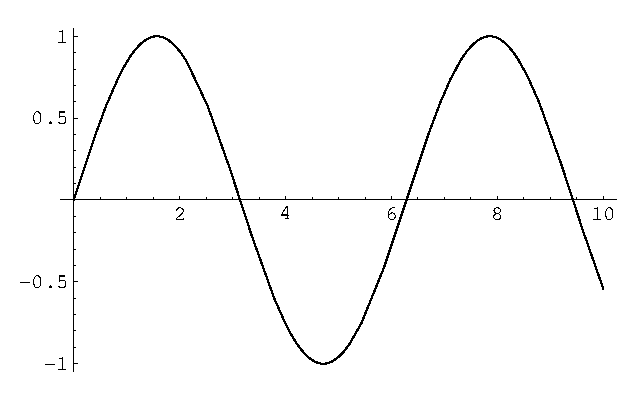
\includegraphics[width=0.8\linewidth]{sample}
	\caption{Sample}
	\label{f:sample}
\end{figure}

see this~\cite{latex}
\section{Background}
\label{s:backg}

\section{Design}
\label{s:design}

\section{Implementation}
\label{s:impl}

\section{Evaluation}
\label{s:eval}

\section{Related work}
\label{s:relwk}
\section{Conclusion}
\label{s:conclusion}

\section{Acknowledgment}
\label{s:ack}



\bibliographystyle{abbrv}
\bibliography{references}

\appendices
\section{Appendix}

This should be Appendix A!


\end{document}
